
\documentclass{cumcmthesis}
    %\documentclass[withoutpreface,bwprint]{cumcmthesis} %去掉封面与编号页

    \usepackage{array} % 用于增强表格功能
    \usepackage{graphicx}  %图片包
    \usepackage{tikz}  %用于画流程图
    \usepackage{flafter} % 在导言区添加这个宏包,使得图片可以更倾向于留在当前位置
    \usepackage{placeins}
    \usepackage{booktabs} % 用于更好的表格线条
    \usepackage{ctex} % 引入ctex宏包,支持中文
    \usepackage{amsmath} % 引入amsmath宏包,支持数学公式
    \usepackage{booktabs} % 用于更好的表格线条
    \usepackage{multirow} % 用于跨行的单元格
    \newcolumntype{C}[1]{>{\centering\arraybackslash}p{#1}} % 自定义列类型,用于居中并设置宽度
    \usetikzlibrary{matrix, arrows, calc} %用于画流程图

    \title{基于ARIMA模型的物料需求预测与生产计划优化}
    \tihao{A}            % 题号
    \baominghao{4321}    % 报名号
    \schoolname{你的大学}
    \membera{成员A}
    \memberb{成员B}
    \memberc{成员C}
    \supervisor{指导老师}
    \yearinput{2024}     % 年
    \monthinput{08}      % 月
    \dayinput{24}        % 日

    \begin{document}
        \maketitle
        \begin{abstract}
            本片论文对于产业上的物料需求问题进行了模型的建立与求解。工业的物料需求是一种时间序列数据,
            我们首先是对不同物料的数据进行分类,将未有需求的空缺值补全为0,即数据的预处理。然后,我们使用了ARIMA
            时间序列模型对数据进行拟合,发现模型对于处于时间序列后期的数据预测效果衰减的程度很大,所以
            我们对模型进行略微的修改,即在每次预测时只预测下一周的数据,下一周时再将下一周的真实数据
            放入训练集中,再次对模型进行拟合。通过对模型的不断更新,最大程度的保证模型的预测能力以及
            对时间序列数据的契合度。\\然后,我们发现模型在预测时,会出现缺货量,库存量交替波动的情况,
            为了保证服务水平,我们引入了安全库存的概念,即在原有的生产计划上适当增加一些生产指标,以
            减少货品缺货的情况,进而提高服务水平。\\然后,我们通过对安全库存的参数调整,以及对模型参
            数的再次网格遍历法,得出服务水平与库存资金相平衡的参数组合,降低了企业可能存在的最大库存
            积压资金。\\最后,对于生产货物的滞后问题,我们对模型先前的循环预测部分进行了逻辑修改,使
            得新的预测部分可以正确计算库存值,正在生产值等。同时,我们也根据ARIMA模型,将其p参数设置
            为2,使得模型中使用了2个单位时间滞后值,符合题目意图。为了使服务水平与库存积压资金相平衡,
            我们重复了第三问的做法,通过不断调整安全库存的参数,ARIMA模型的d,q参数,找出最佳平衡参数
            组合。

            \keywords{时间序列ARIMA模型\quad  单步预测\quad   安全库存}
        \end{abstract}
        \tableofcontents
        \newpage
        \section{问题重述}
        电子产品制造企业面临以下问题:在多品种小批量的物料生产中,事先无法知道物料的
实际需求量。企业希望运用数学方法,分析已有的历史数据,建立数学模型,帮助企业合理地
安排物料生产。
        \subsection{问题一}
        请对历史数据进行分析,选择 6 种应当重点关注的物料(可从物料需求
出现的频数、数量、趋势和销售单价等方面考虑),建立物料需求的周预测模型(即以周为基
本时间单位,预测物料的周需求量),并利用历史数据对预测模型进行评价。
        \subsection{问题二}
        如果按照物料需求量的预测值来安排生产,可能会产生较大的库存,或者出现较
多的缺货,给企业带来经济和信誉方面的损失。企业希望从需求量的预测值、需求特征、库存
量和缺货量等方面综合考虑,以便更合理地安排生产。\\
    请提供一种制定生产计划的方法,从第 101 周开始,在每周初,制定本周的
物料生产计划,安排生产,直至第 177 周为止,使得平均服务水平不低于 85\%。\\    这里假设:本周计划生产的物料,只能在下周及以后使用。为便于统一计算结果,
进一步假设第 100 周末的库存量和缺货量均为零,第 100 周的生产计划数恰好等于第 101 周的
实际需求数。\\
请在问题 1 选定的 6 种物料中选择一种物料,将其第 101 ∼ 110 周的生产计划数、实际
需求量、库存量、缺货量和服务水平按表 1 的形式填写,放在正文中。\\
    请将问题 1 中选定的 6 种物料的全部计算结果(第 101 ∼ 177 周)按表 1 的形式填写在
Excel 文件中,通过支撑材料提交。请将 6 种物料的综合结果(第 101 ∼ 177 周的平均值)按
表 2 的形式填写。
        \subsection{问题三}
        考虑到物料的价格,物料的库存需要占用资金。为了在库存量与服务水平之间达
到某种平衡,如何调整现有的周生产计划,并说明理由。\\    请根据新的周生产计划,对问题 1 选
定的 6 种物料重新计算,并将全部计算结果以表 1 的形式填写在 Excel 表中,通过支撑材料提
交,将综合结果按表 2 的形式填写,放在正文中。对问题 2 选择的 1 种物料,将其第 101 ∼ 110
周的生产计划数、实际需求量、库存量、缺货量和服务水平按表 1 的形式填写,放在正文中。

        \subsection{问题四}
        如果本周计划生产的物料只能在两周及以后使用,请重新考虑问题 2 和问题 3。能
否将你们的方法推广到一般情况,即如果本周计划生产的物料只能在 𝑘 (≥ 2) 周及以后使用,
应如何制定生产计划。
        \section{问题分析}
        \subsection{问题一}
        对于所给的历史数据,我们首先需要对数据进行处理,去除一些总需求量较少的物料,以降低数据的噪声。\\
        然后,我们对预处理的数据使用scikit库作出 周数-需求量 的图,并对每一种物料的需求数据进行快速傅里叶变换分析
        和自相关分析,根据所做出的图标,以及频数,数量,趋势,每周平均销售单价,周期性等选择出 6 种应当重点关注的物料。\\
        \subsection{问题二}
        为了保证服务水平不低于85\%,需要尽量减少缺货的情况,于是可以使用具有防范风险的安全库存模型
        来对模型进行补充,在每次生产时适当增加产量以保证大部分需求能被满足。\\
        \subsection{问题三}
        由于第二问只考虑了服务水平,没有考虑到库存的积压资金,所以我们先对库存积压资金做出定义,然后再对安全库存
        参数做出调整,以减少库存积压资金的同时保证服务水平。\\

        \subsection{问题四}
        我们先根据ARIMA模型的参数性质,对p参数进行调整,即模型可以使用p个单位时间滞后值,然后再对安全库存参数做出
        遍历分析,找出最佳的平衡参数组合。\\
        \section{模型的假设}
        我们假定:\\
        \begin{itemize}
            \item 对于第i周的数据未有提及,则第i周的需求量为0,销售单价为NULL。
            \item 对于第i周的缺货量,会加入原本第i+1周的需求量成为第i+1周的实际需求量。
            \item 所有物料的数量,供需数量都为0或正整数。
            \item 对于库存物料的积压资金,等于该周货物的多余量*平均单价。
        \end{itemize}
        
        \section{符号说明}
        \begin{center}
            \begin{tabular}{cc}
                \hline
                \makebox[0.3\textwidth][c]{符号}	&  \makebox[0.4\textwidth][c]{意义} \\ \hline
                $SS$	    & 安全库存(件) \\ \hline
                $Z$	    & 安全系数 \\ \hline
                $\sigma_{LT}$	    & 需求量的标准差 \\ \hline
            \end{tabular}
        \end{center}
        \section{模型的建立与求解}
        \subsection{问题一}
        对于预处理好的数据,我们先通过总需求次数是否大于20来将需求量过于小的物料排除;然后对剩下的物料数据作出 周数-需求量
         周数-销售单价 周数-盈利 的折线图,通过分析再进一步排除需求出现较大空窗期的物料;然后再对剩下的物料作出简单的快速傅里叶变换
        分析,自相关分析判断其是否具有一定周期性。同时,使用python库statsmodels对物料的需求量进行多项式回归、指数平滑模型、
        时间序列模型进行简单拟合,初步判断物料需求量函数拟合的可行性。\\

        \begin{figure}[ht]
            \centering
            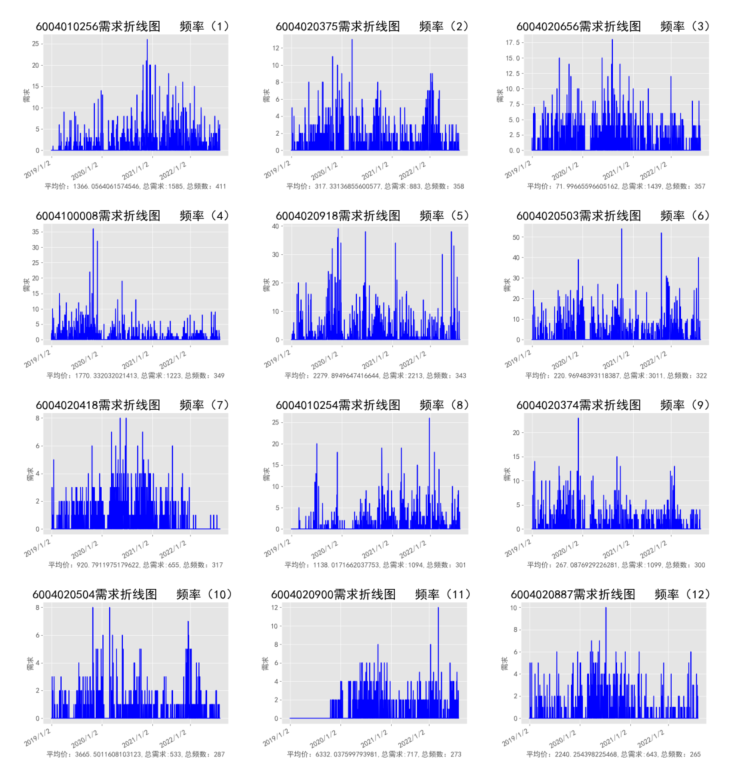
\includegraphics[width=\textwidth]{graph/graph_1.png}
            \caption{12种预选的物料频率图}
            \label{fig:1}
        \end{figure}

        对于企业来说,肯定是希望做一些需求更稳定的,需求量少,而销售单较高的物料来进行生产。为此我们从以上的12中物料中
        选取了6004010256、6004020656、6004100008、6004020918、6004020503、6004020900这6种物料进行进一步分析。\\其中,6004010256、
        6004100008、6004020900的单价较高;6004020656、6004010256、6004020503的需求量大;6004020918、6004020900的
        平均单价稳定。

        \iffalse % 开始多行注释
        物料编码:6004010256  单价高,需求多,收益高
        ADF Statistic: -2.9016997826218742
        p-value: 0.045150692630650704
        数据在0阶差分后平稳。
        基于AIC选择的最佳ARIMA模型: ARIMA(4, 0, 4) - AIC:1003.3296543735466
        基于BIC选择的最佳ARIMA模型: ARIMA(1, 0, 3) - BIC:1026.8280437872822

        物料编码:6004020656  需求多
        ADF Statistic: -4.689966353402755
        p-value: 8.788187042947568e-05
        数据在0阶差分后平稳。
​        基于AIC选择的最佳ARIMA模型: ARIMA(1, 0, 1) - AIC:952.1385872328146
        基于BIC选择的最佳ARIMA模型: ARIMA(1, 0, 1) - BIC:964.2077065800744


        物料编码:6004100008  需求量很低,但是单价高,收益一般
        ADF Statistic: -2.917519046355061
        p-value: 0.04334837036103692
        数据在0阶差分后平稳。
        基于AIC选择的最佳ARIMA模型: ARIMA(1, 0, 2) - AIC:930.7906642414423
        基于BIC选择的最佳ARIMA模型: ARIMA(1, 0, 2) - BIC:945.5344636933331

        物料编码:6004020918  价格很稳定,但是需求起伏大,有一定的周期性
        ADF Statistic: -4.488954310407512
        p-value: 0.00020587696294737737
        数据在0阶差分后平稳。
        基于AIC选择的最佳ARIMA模型: ARIMA(3, 0, 0) - AIC:1155.9054549407583
        基于BIC选择的最佳ARIMA模型: ARIMA(1, 0, 1) - BIC:1168.1920469180693

        物料编码:6004020503  量大
        ADF Statistic: -4.51920635549633
        p-value: 0.00018150974951260178
        数据在0阶差分后平稳。
        基于AIC选择的最佳ARIMA模型: ARIMA(0, 0, 3) - AIC:1165.501744798226
        基于BIC选择的最佳ARIMA模型: ARIMA(0, 0, 0) - BIC:1176.6331343686945

        物料编码 :6004020900
        ADF Statistic: -2.019088771208017
        p-value: 0.27826656262718763
        ADF Statistic: -9.485036789747918
        p-value: 3.7827402197577234e-16
        数据在1阶差分后平稳。
        基于AIC选择的最佳ARIMA模型: ARIMA(4, 1, 4) - AIC:587.6768266346218
        基于BIC选择的最佳ARIMA模型: ARIMA(0, 1, 1) - BIC:594.1890466728535

        \fi % 结束多行注释

        \iffalse % 开始多行注释
        \begin{table}[h]
            \centering
            \caption{ADF检验结果汇总}
            \label{tab:ADF_results}
            \begin{tabular}{|c|c|c|}
            \hline
            \textbf{物料编码} & \textbf{ADF Statistic} & \textbf{p-value} \\ \hline
            6004010256 & -2.9017 & 0.0452 \\
            6004020656 & -4.6900 & 0.0000879 \\
            6004100008 & -2.9175 & 0.0434 \\
            6004020918 & -4.4890 & 0.0002059 \\
            6004020503 & -4.5192 & 0.000182 \\
            6004020900 & -9.4850 & 3.7827e-16 \\ \hline
            \end{tabular}
        \end{table}
        \fi % 结束多行注释

        我们先对数据进行了ADF测试,判断数据是否平稳,然后对进行了差分的具有平稳性的数据
        使用BIC(贝叶斯信息准则),AIC(赤池信息准则)计算选出最佳的p,d,q参数组合。
        然后我们将70\%的总数据作为训练集,30\%的数据作为测试集,在训练集上
        用得到的参数进行了基于最大似然估计的ARIMA模型的拟合,得到了最佳的ARIMA模型。
        接着使用模型对测试集进行预测,绘制出 预测——周数、实际值——周数 的二维图如下。\\

        \begin{figure}[ht]
            \centering
            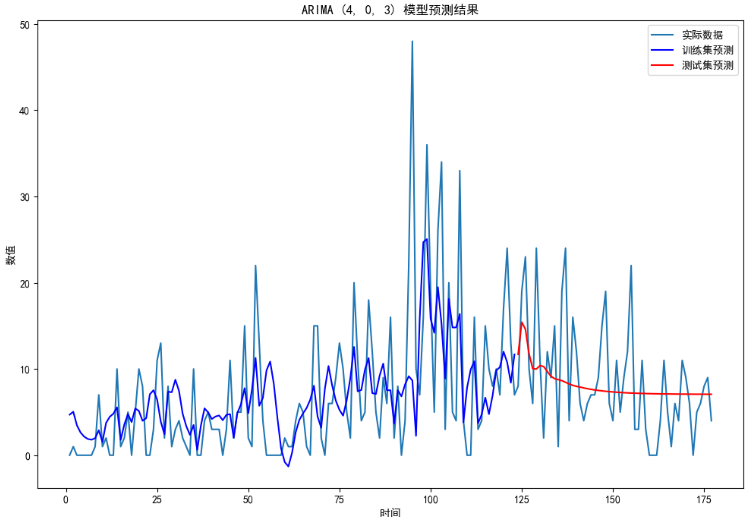
\includegraphics[scale=0.8]{graph/graph_2.png}
            \caption{物料编码:6004010256}
            \label{fig:2}
        \end{figure}
        \FloatBarrier    %使用这个命令使得图片不会浮动到下一页
        
        如上图片,我们发现,ARIMA模型在训练集上的表现还比较好,但是在测试集上的表现出现较大偏差
        模型对于前期部分的测试数据的预测仍能基本跟上真实值的变化趋势,但是对于后期的数据预测效果较差,
        预测曲线基本趋平。于是,我们决定对ARIMA模型的预测部份进行修改,使它可以进行循环的“单步预测”,具体如下:\\
        
        
        \iffalse % 开始多行注释
        \begin{figure}[ht]
            \centering
            \begin{minipage}{0.4\textwidth}
                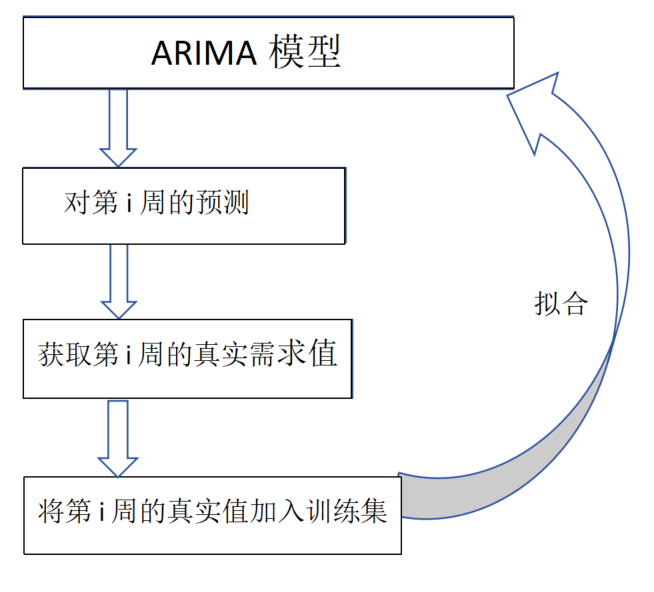
\includegraphics[width=\linewidth]{graph/graph_3.png}
                \caption{“循环单步预测”示意图}
                \label{fig:temp}
            \end{minipage}%
            \hfill % 增加一些水平空间
            \begin{minipage}{0.55\textwidth}
                % 文字描述
                我们先用前70\%的数据进行拟合,然后使用ARIMA模型对下一周进行预测,等到下一周获取到真实值后,将
                下一周的真实值加入到训练集中,再次使用ARIMA模型进行拟合,再对下下周进行预测,如此循环往复。即每次
                模型只对下一周进行与预测,极大的保证了模型的性能优势与准确性。\\
            \end{minipage}
        \end{figure}

        \fi % 结束多行注释

        %\vspace{10pt}   %添加图片到上下文字的前后距离
        \begin{figure}[ht!]
            \centering
            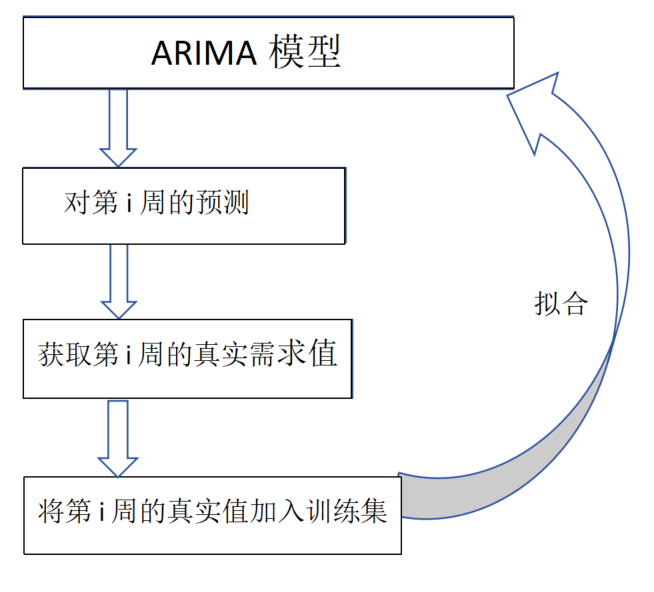
\includegraphics[scale=0.7]{graph/graph_3.png}
            \caption{“循环单步预测”示意图}
            \label{fig:3}
        \end{figure}
        %\vspace{10pt}
        \FloatBarrier    %使用这个命令使得图片不会浮动到下一页

        我们先用前70\%的数据进行拟合,然后使用ARIMA模型对下一周进行预测,等到下一周获取到真实值后,将
        下一周的真实值加入到训练集中,再次使用ARIMA模型进行拟合,再对下下周进行预测,如此循环往复。即每次
        模型只对下一周进行与预测,极大的保证了模型的性能优势与准确性。以下是我们使用了“循环单步预测”后的预测
        图像:\\


        %我想要搞一个四宫格
        \begin{figure}[ht]
            \centering
            \begin{subfigure}[b]{0.49\textwidth}
                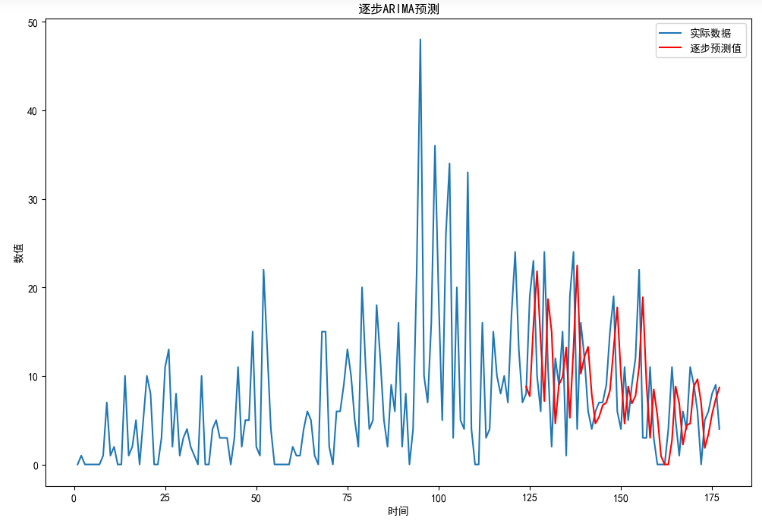
\includegraphics[width=\textwidth]{graph/graph_4.png}
                \caption{预测值与实际值对比图}
                \label{fig:image1}
            \end{subfigure}
            \hfill % 插入水平间距
            \begin{subfigure}[b]{0.49\textwidth}
                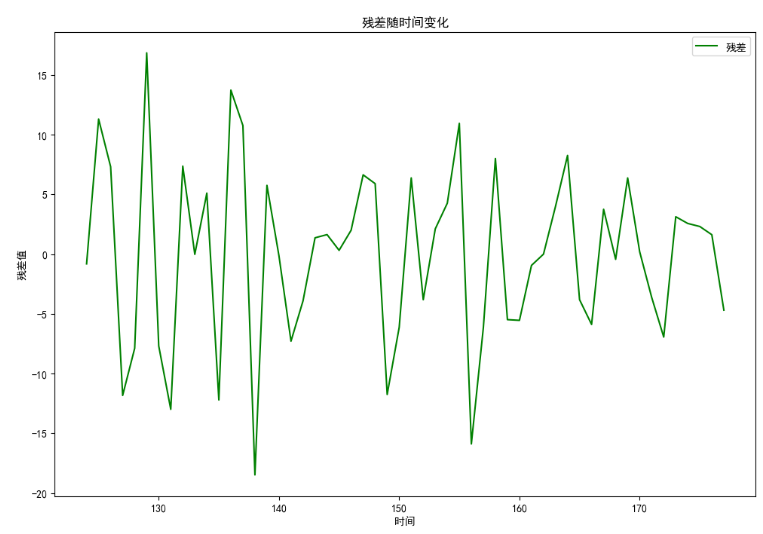
\includegraphics[width=\textwidth]{graph/graph_7.png}
                \caption{模型残差图}
                \label{fig:image2}
            \end{subfigure}

            \begin{subfigure}[b]{0.49\textwidth}
                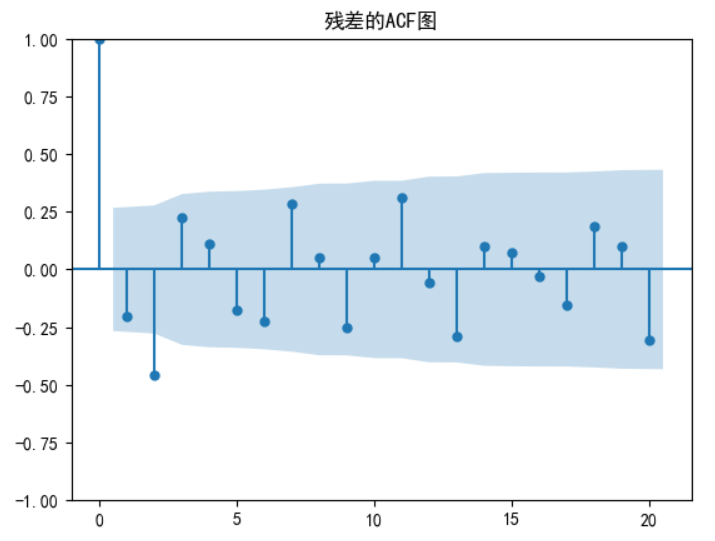
\includegraphics[width=\textwidth]{graph/graph_6.png}
                \caption{模型残差自相关ACF图}
                \label{fig:image3}
            \end{subfigure}
            \hfill % 插入水平间距
            \begin{subfigure}[b]{0.49\textwidth}
                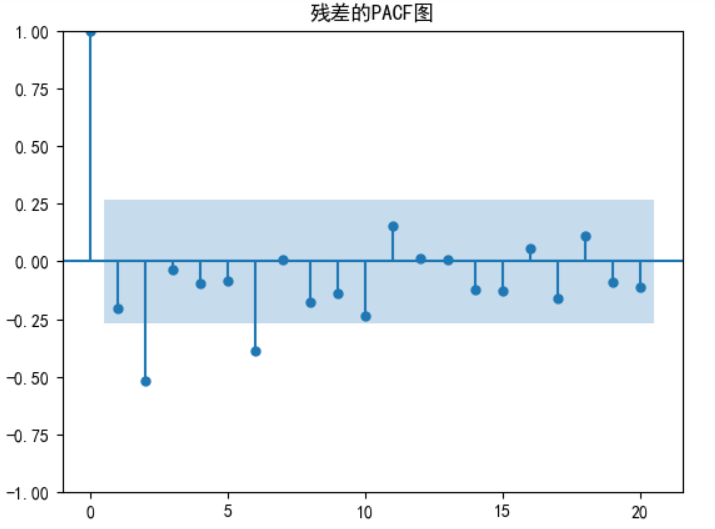
\includegraphics[width=\textwidth]{graph/graph_5.png}
                \caption{模型残差正态分布PACF图}
                \label{fig:image4}
            \end{subfigure}
        \end{figure}


        可以看到,我们通过“循环单步预测”得到的ARIMA模型可以预测需求的趋势,且较为准确,
        预测曲线与实际需求曲线基本重合。同时,模型的残差图中的残差分布随机,没有明显的模式或者趋势
        。ACF与PACF图中的值都是从1.0快速衰减到零区间附近,但也存在小部分“异常值”,尽管如此,所有的
        数值都是处于置信区间内,证明了“循环单步预测”ARIMA模型在对物料需求上的预测准确性。\\
        \\
        于是,我们将每个物料都进行了ARIMA模型的拟合,并使用循环的单步预测法进行预测,得到的结果如下:\\
        
        \begin{figure}[ht]
            \centering
            \begin{subfigure}[b]{0.49\textwidth}
                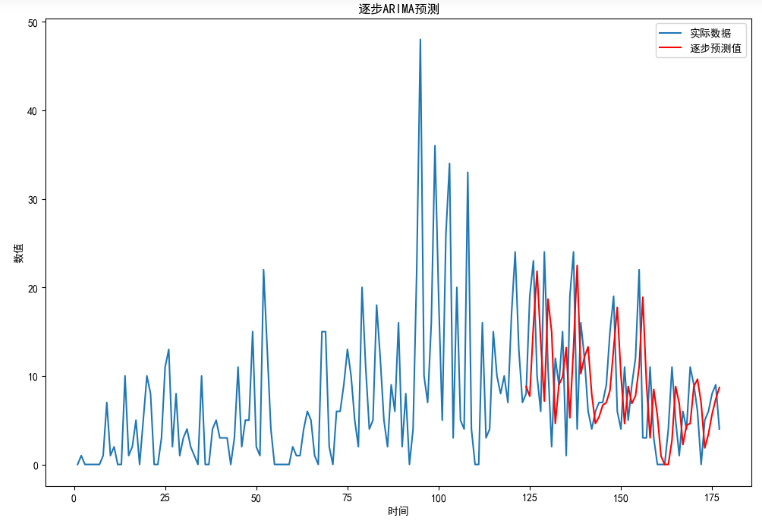
\includegraphics[width=0.8\textwidth]{graph/graph_4.png}
                \caption{物料编码:6004010256}
                \label{fig:image1}
            \end{subfigure}
            \hfill % 插入水平间距
            \begin{subfigure}[b]{0.49\textwidth}
                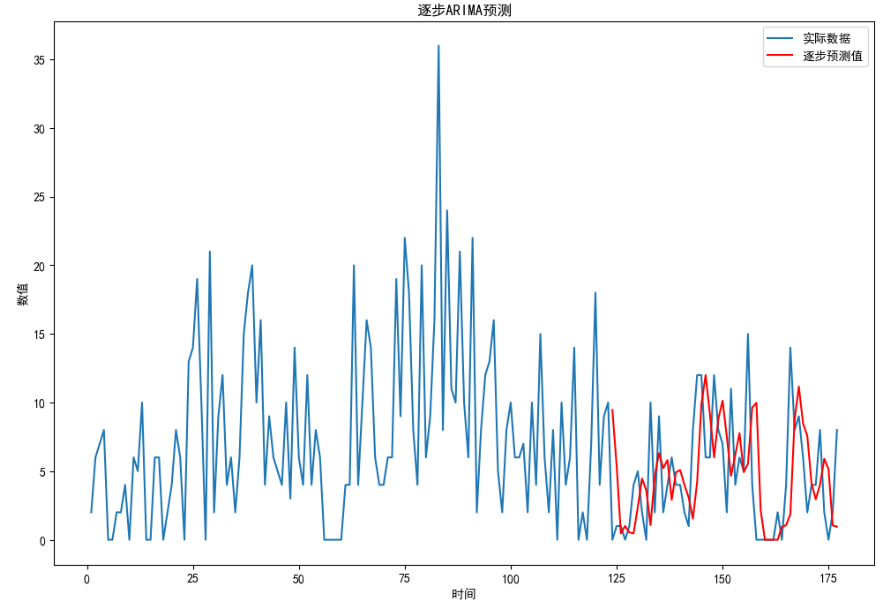
\includegraphics[width=0.8\textwidth]{graph/graph_12.png}
                \caption{物料编码:6004020656}
                \label{fig:image2}
            \end{subfigure}

            \begin{subfigure}[b]{0.49\textwidth}
                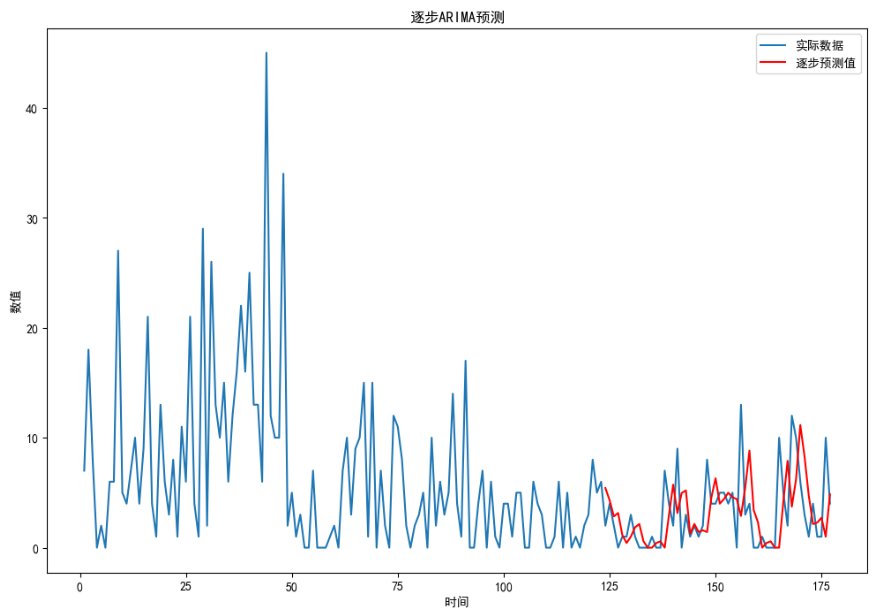
\includegraphics[width=0.8\textwidth]{graph/graph_11.png}
                \caption{物料编码:6004100008}
                \label{fig:image3}
            \end{subfigure}
            \hfill % 插入水平间距
            \begin{subfigure}[b]{0.49\textwidth}
                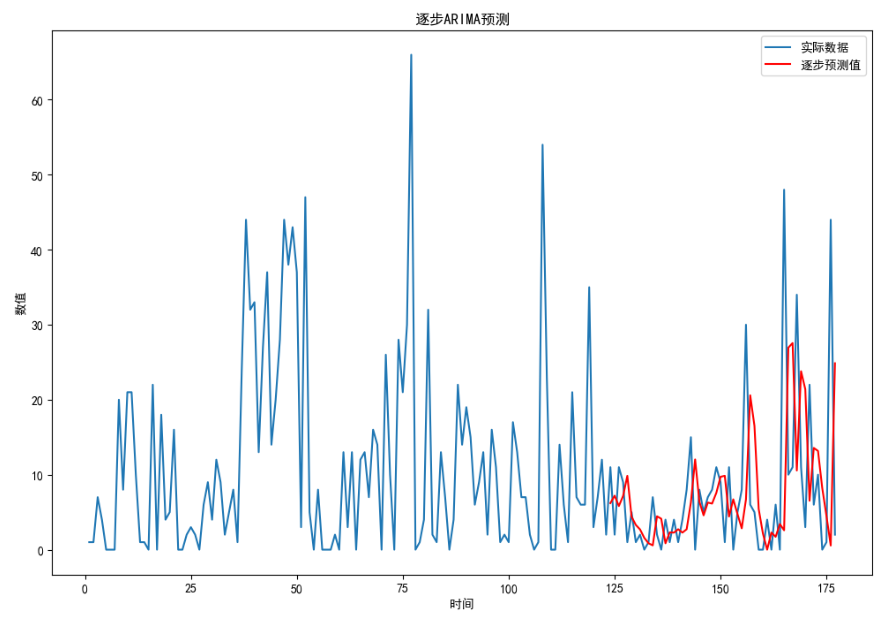
\includegraphics[width=0.8\textwidth]{graph/graph_10.png}
                \caption{物料编码:6004020918}
                \label{fig:image4}
            \end{subfigure}

            \begin{subfigure}[b]{0.49\textwidth}
                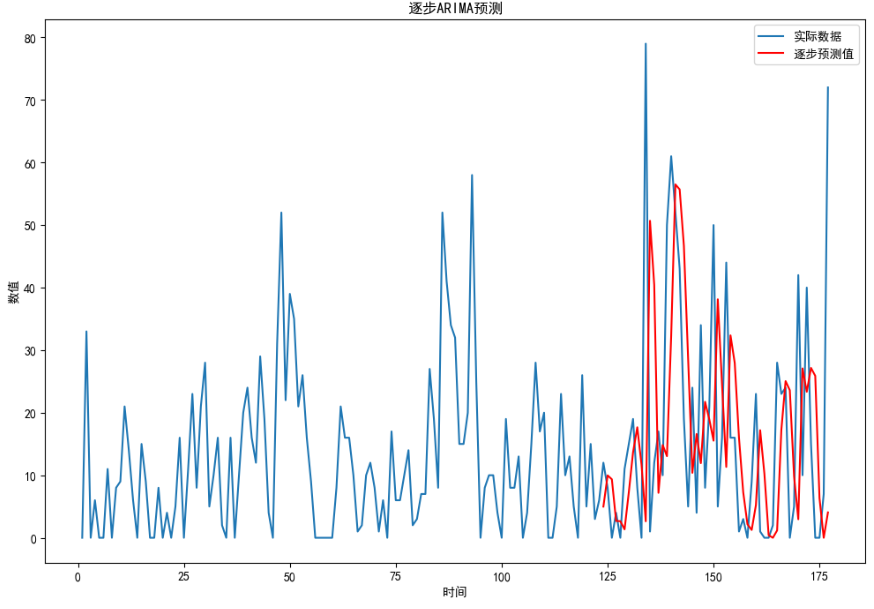
\includegraphics[width=0.8\textwidth]{graph/graph_9.png}
                \caption{物料编码:6004020503}
                \label{fig:image5}
            \end{subfigure}
            \hfill % 插入水平间距
            \begin{subfigure}[b]{0.49\textwidth}
                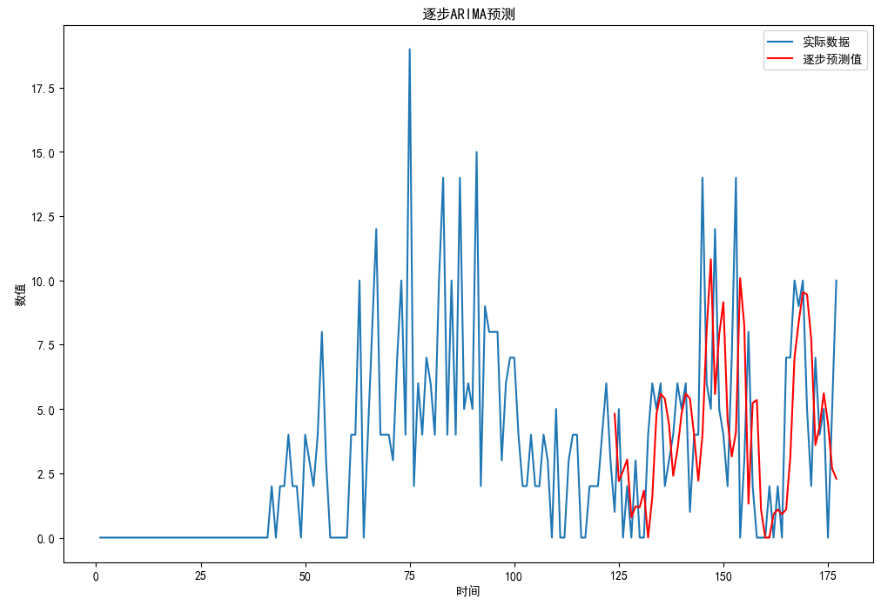
\includegraphics[width=0.8\textwidth]{graph/graph_8.png}
                \caption{物料编码:6004020900}
                \label{fig:image6}
            \end{subfigure}
        \end{figure}
        \FloatBarrier    %使用这个命令使得图片不会浮动到下一页

        \subsection{问题二}
        题目要求从第101周开始预测,于是我们更改训练集与测试集,继续使用第一问得到的循环单步预测法进行预测。
        同时记录下缺货量,库存量等信息,如下:\\
        
        \begin{figure}[ht]
            \centering
            \begin{subfigure}[b]{0.49\textwidth}
                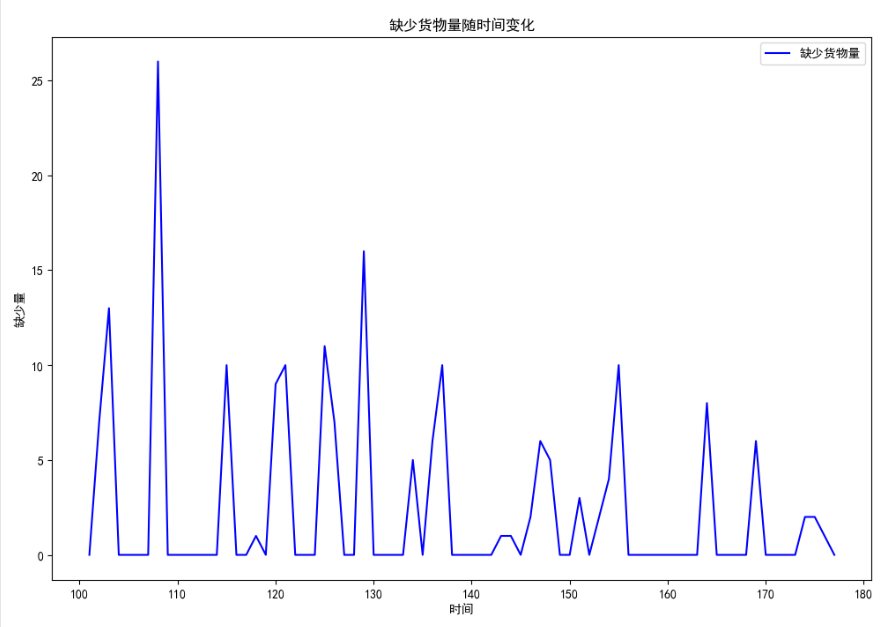
\includegraphics[width=0.8\textwidth]{graph/graph_15.png}
                \caption{缺失值}
                \label{fig:image1}
            \end{subfigure}
            \hfill % 插入水平间距
            \begin{subfigure}[b]{0.49\textwidth}
                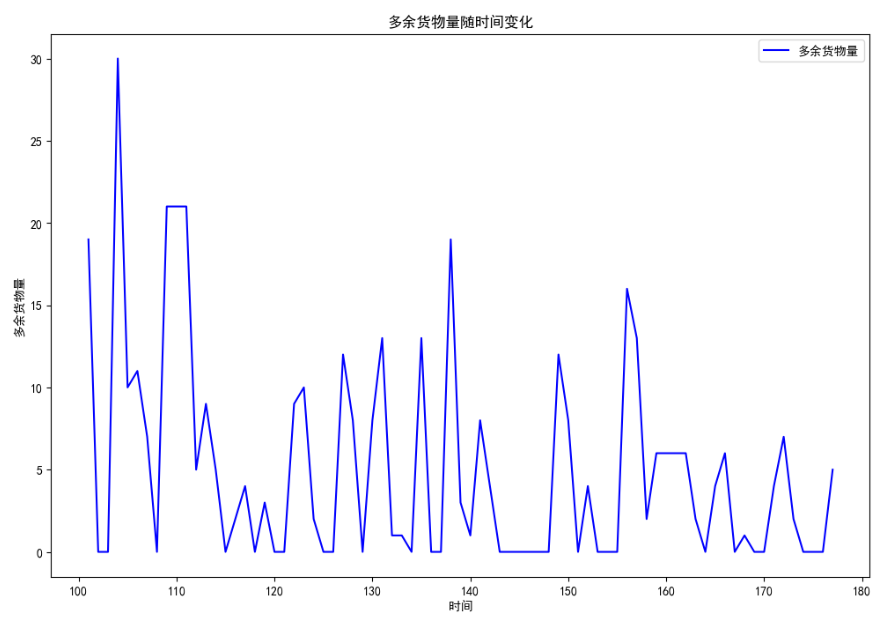
\includegraphics[width=0.8\textwidth]{graph/graph_16.png}
                \caption{库存值}
                \label{fig:image2}
            \end{subfigure}
        \end{figure}

        我们发现,对于大部分物料来说,缺货量与库存量总是处于较为随机的交替起伏的情况下,即使平均服务的水平
        达到了85\%,但是缺货量与库存量的波动仍然较大,这对于企业的信誉来说是不利的。于是,我们在预测的同时加入了
        安全库存的概念,可以在原有预测生产的基础上,适当增加一些生产指标,以增加企业面对突变的需求量的抗风险能力。\\

        \[
        SS = Z \times \sigma_{LT}
        \]
        其中,$SS$为安全库存,$Z$为安全系数,$\sigma_{LT}$为需求量的标准差。\\

        \iffalse % 开始多行注释
        \begin{figure}[ht!]
            \centering
            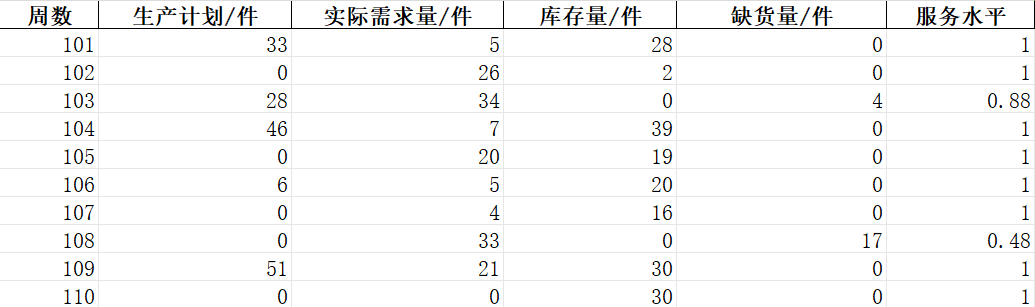
\includegraphics[width=0.8\textwidth]{graph/graph_14.png}
            \caption{6004010256物料第 101~110 周的生产计划、实际需求、库存、缺货量及服务水平}
            \label{fig:13}
        \end{figure}
        \fi % 结束多行注释
        
        \begin{table}[htbp]
            \centering
            \small % 减小字体大小
            \begin{tabular}{cccccc}
            \toprule
            周数 & 生产计划/件 & 实际需求量/件 & 库存量/件 & 缺货量/件 & 服务水平 \\
            \midrule
            101 & 33 & 5 & 28 & 0 & 1.0 \\
            102 & 0 & 26 & 2 & 0 & 1.0 \\
            103 & 28 & 34 & 0 & 4 & 0.88 \\
            104 & 46 & 7 & 39 & 0 & 1.0 \\
            105 & 0 & 20 & 19 & 0 & 1.0 \\
            106 & 6 & 5 & 20 & 0 & 1.0 \\
            107 & 0 & 4 & 16 & 0 & 1.0 \\
            108 & 0 & 33 & 0 & 17 & 0.48 \\
            109 & 51 & 21 & 30 & 0 & 1.0 \\
            110 & 0 & 0 & 30 & 0 & 1.0 \\
            111 & 0 & 0 & 30 & 0 & 1.0 \\
            \bottomrule
            \end{tabular}
            \caption{6004010256物料第 101~110 周的生产计划、实际需求、库存、缺货量及服务水平}
            \label{tab:prod_inv_data} % 为表格添加引用标签
            \footnotetext{我们可以看到,在使用了安全库存之后,整体满意度处于高位。} % 添加脚注
        \end{table}
        \FloatBarrier    %使用这个命令使得图片不会浮动到下一页
        
        于是,在使用了安全库存之后,我们的平均满意度可以达到较高的水平。

        \subsection{问题三}

        对于题目所说的物料积压资金,我们认为可以用最大库存量时的所需最大库存积压资金来衡量模型预测在
        物料积压资金上面的水平。\\
        \begin{equation}
            \text{物料数量} \times \text{平均单价} = \text{所需最大库存积压资金}
        \end{equation}
        因为对于企业来说,一般生产的预备资金是一直用于某个物料上的,不会流动,即增加或者减少。所以
        我们认为 所需最大库存积压资金 就代表了企业可以只放置这么多资金在这个物料上,就能保证货物正常
        生产以及积压。\\
        为了计算物料库存的积压资金,我们先对无物料的前100周的平均价格数据进行了分析,以下以物料编码
        6004010256的物料为例:\\
        我们对物料前100周的价格数据进行了简单的统计分析和画图,发现价格在前55周处于相对波动的范围,
        在后56周至100周则相对稳定,由于我们计算的是第101周至177周的预算与货物的积压资金,所以我们
        选择使用后45周的平均价格作为计算货物积压的平均价格,即1483.1元。\\
        在此基础上,以物料6004010256为例子,我们计算了物料库存的积压资金,如下:\\

        \begin{figure}[ht!]
            \centering
            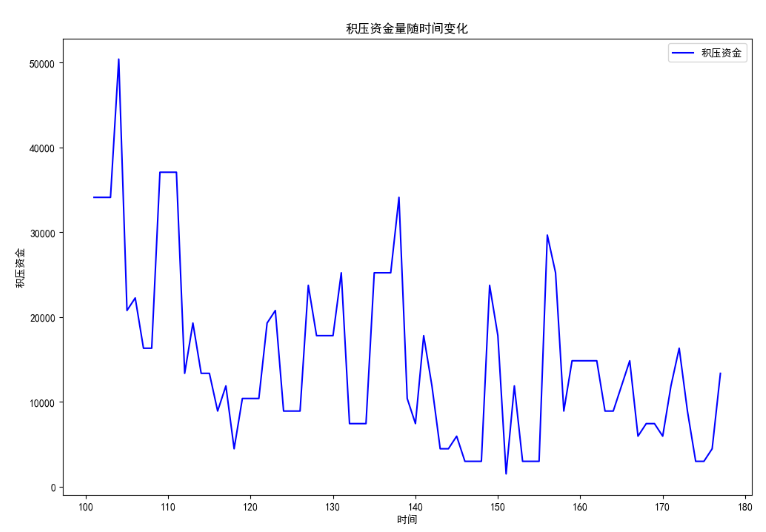
\includegraphics[width=0.8\textwidth]{graph/graph_17.png}
            \caption{6004010256物料在使用第二问模型下的 库存积压资金-时间 图}
            \label{fig:17}
        \end{figure}

        通过如上的图片,我们发现由于安全库存的设定导致我们的库存量基本保持在1以上,而且峰值也远高于
        大部分需求的值,这也就使得物料的库存积压资金过高,不符合企业的低资金积压目标。所以我们重新通
        过网格遍历法以及调整安全库存的服务满意度大小来调整生产计划。具体来说,我们重新通过网格遍历法
        搜索计算,先在每一种参数组合下求出最大的资金挤压值,然后对比每一组参数的最大资金积压值,选取
        最小的那一组参数作为最终的参数组合。\\

        但是我们发现这样还不够,由于安全库存的影响过于强烈,导致我们的库存量过高,所以我们对安全库存
        的服务水平参数进行了调整,使得安全库存的影响减弱,同时保证题目中随定义的服务水平。\\

        \begin{table}[htbp]
            \centering
            \caption{物料:6004010256 的 安全库存与服务水平和最大库存积压资金的关系}
            \label{tab:safety_stock}
            \begin{tabular}{ccc} % 3列
            \toprule
            安全库存 & 服务水平 & 最大库存积压资金 \\
            \midrule
            0 & 0.8946935172146779 & 28178.9 \\
            1 & 0.900971134024425 & 19280.3 \\
            2 & 0.9167137896136947 & 19280.3 \\
            3 & 0.9271877899399739 & 20763.4 \\
            4 & 0.9391972779102511 & 22246.5 \\
            5 & 0.9483656639510848 & 23729.6 \\
            6 & 0.9568084614732336 & 25212.7 \\
            7 & 0.9636698282973934 & 26695.8 \\
            \bottomrule
            \end{tabular}
        \end{table}

        可以看到,对于任意的安全库存值来说,服务水平都是在85\%以上,但是随着安全库存的增加,最大库存积压资金
        会有些许不同,于是我们在保证服务水平尽可能高的情况下,选择安全库存的货物数量为2。对于剩下的物料,我们
        也是先观察他们每周价格的波动情况,求出相对客观的平均价格;然后通过网格搜索求出最大库存资金中最小的的
        p,d,q参数值,最后遍历安全库存的大小,选择最大库存资金中最小的安全库存量即可。\\


        \subsection{问题四}

        我们使用了基于平均需求和供应提前期的安全库存的双步预测模型,即将原本模型的经典安全库存模型
        更改为基于平均需求和供应提前期的安全库存模型,将原本的每次只对下一周进行预测变为对下两周进
        行预测。并且对第101周和第177周的预测与计算进行了特殊处理。以此来适应题目的要求。\\

        具体来说,我们在每一个单步预测的循环内:
        \begin{enumerate}
            \item 对第i周和第i+1周的需求量进行预测。
            \item 通过预测计算第i-1周要生产的物料数量。
            \item 获取第i周的实际需求量,计算第i周的缺货量,存货量。
            \item 更新库存,加上第i-1周的上产量。
            \item 重复1-4步骤。
        \end{enumerate}

        \begin{align}
            &\quad\text{第} (i-1) \text{周要生产的物料数量} \notag \\
            &\quad= \text{第} i \text{周的预测值} + \text{第} (i+1) \text{周的预测值} - \text{安全库存} - \text{库存(现有的可以用的货物)}
        \end{align}

        按照上述的步骤,我们更新了代码模块,重新进行了模型的拟合,得到了新的预测结果,
        如下图:\\

        \begin{figure}[ht!]
            \centering
            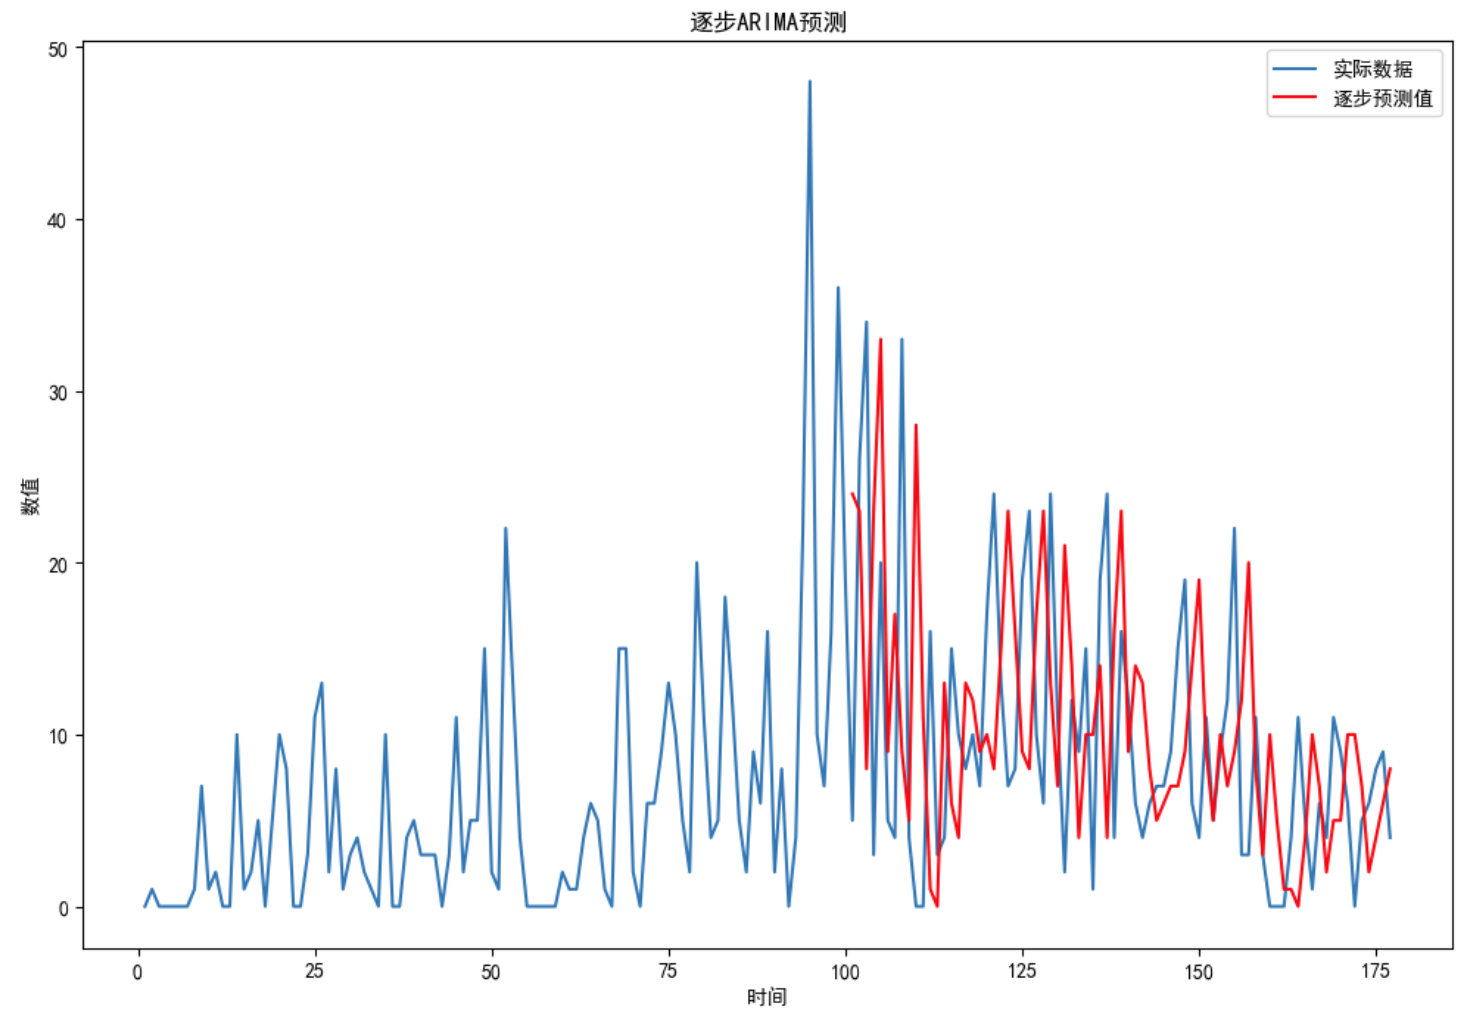
\includegraphics[width=0.8\textwidth]{graph/graph_18.png}
            \caption{6004010256物料在考虑生产滞后性的 预测-时间 图}
            \label{fig:18}
        \end{figure}
        \FloatBarrier    %使用这个命令使得图片不会浮动到下一页

        通过如上的图片,我们发现,我们的模型在考虑了生产滞后性后,预测的效果依然较好,预测曲线与实际需
        求曲线基本重合,并且计算得出其服务水平参数为:88.9\%,满足第二问对服务水平的要求。\\

        同时,我们将我们先前的ARIMA模型的 p 参数进行了修改,将其值设定为2。因为在ARIMA模型中,p参数
        表示模型中使用了多少个时间滞后值。例如,如果 p=1,则模型会考虑前一期的值作为当前值的预测因素。
        我们将它设为2则可以符合题目条件要求“本周计划生产的物料只能在两周及以后使用”。但是实验数据却显示
        对于相同的d,q参数,p=3的模型的平均服务水平和最大物料积压资金值要优于p=1,p=2,p=4的模型。
        此时,我们也对安全库存的数量进行了遍历,与p参数一起进行。最终我们
        选择了表现最佳的p=3,与安全库存数量=6,(注:3倍平均需求量的库存积压值为31145.1)具体如下:\\

        \begin{table}[htbp]
            \centering
            \caption{物料6004010256在不同安全库存条件,不同p值下的最大库存积压资金与服务水平}
            \label{tab:safety_stock_data}
            
            \begin{tabular}{cccC{2cm}C{2cm}} % 设置列的对齐和宽度
            \toprule
             & 安全库存数量 & 最大库存积压资金 & 服务水平 \\
            \midrule
            \multirow{8}{*}{p,d,q=(2,1,1)} % 211 的数据跨8行
                & 0 & 57840.9 & 0.8396 \\
                & 1 & 45976.1 & 0.8342 \\
                & 2 & 43009.9 & 0.8559 \\
                & 3 & 43009.9 & 0.8725 \\
                & 4 & 41526.8 & 0.8894 \\
                & 5 & 41526.8 & 0.9042 \\
                & 6 & 43009.9 & 0.9110 \\
                & 7 & 44493.0 & 0.9196 \\
            \midrule
            \multirow{8}{*}{p,q,d=(3,1,1)}
                & 0 & 60807.1 & 0.8374 \\
                & 1 & 48942.3 & 0.8517 \\
                & 2 & 34111.3 & 0.8604 \\
                & 3 & 34111.3 & 0.8768 \\
                & 4 & 35594.4 & 0.8893 \\
                & 5 & 37077.5 & 0.8997 \\
                & 6 & 38560.6 & 0.9075 \\
                & 7 & 40043.7 & 0.9132 \\
            \midrule
            \multirow{8}{*}{p,q,d=(4,1,1)}
                & 0 & 60807.1 & 0.8374 \\
                & 1 & 48942.3 & 0.8472 \\
                & 2 & 37077.5 & 0.8615 \\
                & 3 & 37077.5 & 0.8738 \\
                & 4 & 38560.6 & 0.8886 \\
                & 5 & 37077.5 & 0.8977 \\
                & 6 & 38560.6 & 0.9054 \\
                & 7 & 40043.7 & 0.9135 \\
            \bottomrule
            \end{tabular}
        \end{table}
        \FloatBarrier    %使用这个命令使得图片不会浮动到下一页
        
        在确保物料6004010256在生产滞后情况下的模型求解后,我们依照此思路对剩余的物料进行了模型求解,
        得到的结果如下:\\

        \begin{table}[htbp]
            \centering
            \caption{六种物料的示意表格}
            \label{tab:example-data}
            
            \begin{tabular}{cccc} % 4列,列顺序调整为:编码、序号、库存积压资金、服务水平
            \toprule
            物料编码 & 安全库存量 & 最大库存积压资金 & 平均服务水平 \\
            \midrule
            6004010256 & 6 & 38560.6 & 0.9075 \\
            6004020656 & 3 & 25212.7 & 0.9018 \\
            6004100008 & 4 & 17797.2 & 0.9004 \\
            6004020918 & 13 & 56357.8 & 0.9039 \\
            6004020503 & 16 & 75638.1 & 0.9010 \\
            6004020900 & 2 & 22246.5 & 0.9012 \\
            \bottomrule
            \end{tabular}
        \end{table}

        对于不同的物料,使用相同的我们的基于ARIMA时间序列模型的代码进行求解,最终获得低于4倍的
        平均需求量的最大积压资金,并且平均服务水平均达到90\%以上,我们认为我们的预测模型具有一般性
        ,即可以将我们的模型扩展到一般情况。对于不同的物料我们可以通过修改ARIMA模型的相关参数,
        或者对安全库存进行修改来对实际的情况进行拟合,最终达到较好效果。\\

        \section{总结}
        本文首先对物料的需求量等数据进行了数据预处理,然后进行了ARIMA模型的拟合,接着通过循环单步
        预测法对需求量进行了预测,运用了ADF验证等方式,说明了预测的准确性。然后我们引入了安全库存的
        概念,调整安全库存使得平均服务水平达到85\%以上。接着通过调整安全库存的大小,以及对参数的
        调整,我们可以使得物料的最大库存积压资金达到最小,同时保证服务水平,达到了服务水平与积压资金
        的平衡。最后,我们对先前的ARIMA模型预测部份进行微调,使得模型可以适应生产滞后的情况,并借用
        第二三问思路,对安全库存量与参数进行遍历,得到服务水平与积压资金平衡的参数组合。最终在6种
        物料上进行了拟合,均达到很好效果,也说明了我们模型对于一般情况的适应性,即具有一般性。\\
        \begin{thebibliography}{9}%宽度9
            \bibitem{bib:one} ....
        \end{thebibliography}
        \begin{appendices}
            附录内容。
        \end{appendices}
    \end{document}